\documentclass[12pt,a4paper]{report}
\usepackage[utf8]{inputenc}
\usepackage[english]{babel}
\usepackage[T1]{fontenc}
\usepackage{geometry}
\usepackage{setspace}
\usepackage{graphicx}
\usepackage{hyperref}
\usepackage{listings}
\usepackage{xcolor}
\usepackage{float}
\usepackage{caption}
\usepackage{subcaption}

% Page configuration
\geometry{left=3cm, right=2cm, top=2.5cm, bottom=2.5cm}
\onehalfspacing

% Hyperref configuration
\hypersetup{
    colorlinks=true,
    linkcolor=black,
    filecolor=magenta,      
    urlcolor=blue,
    citecolor=black
}

% Code listings configuration
\lstset{
    basicstyle=\ttfamily\small,
    keywordstyle=\color{blue},
    commentstyle=\color{green!60!black},
    stringstyle=\color{red},
    showstringspaces=false,
    breaklines=true,
    frame=single,
    backgroundcolor=\color{gray!10}
}

\begin{document}

% Title page (according to Annex 3)
\begin{titlepage}
    \centering
    {\Large \textbf{ALEXANDRU IOAN CUZA UNIVERSITY OF IAȘI}}\\[0.5cm]
    {\Large \textbf{FACULTY OF COMPUTER SCIENCE}}\\[2cm]
    
    {\Huge \textbf{Off Course - Web Platform for Exploring Abandoned Buildings in Romania}}\\[3cm]
    
    {\Large Popa Cosmin-George}\\[2cm]
    
    {\large Session: July, 2025}\\[2cm]
    
    {\large Scientific Supervisor}\\
    {\large Prof. Dr. Pătruț Bogdan}\\[2cm]
    
    \vfill
    {\large Iași}\\
    {\large 2025}
\end{titlepage}

% Declarations (according to annexes 4 and 5)
\chapter*{Declaration of Originality}
\addcontentsline{toc}{chapter}{Declaration of Originality}

I, Popa Cosmin-George, domiciled in [address], born on [date], identified by CNP [CNP], graduate of Alexandru Ioan Cuza University of Iași, Faculty of Computer Science, specialization Computer Science in English, class of 2025, declare on my own responsibility, knowing the consequences of false statements under art. 326 of the New Penal Code and the provisions of the National Education Law no. 1/2011 art.143 par. 4 and 5 regarding plagiarism, that the bachelor's thesis entitled:

\textbf{Off Course - Web Platform for Exploring Abandoned Buildings in Romania}

developed under the guidance of Prof. Dr. Pătruț Bogdan, which I will present before the commission is original, belongs to me and I assume full responsibility for its content.

I also declare that I agree that my bachelor's thesis may be verified by any legal means to confirm its originality, including consenting to the introduction of its content into a database for this purpose.

\vspace{2cm}
Date: [date] \hfill Student signature

\newpage

\chapter*{Declaration of Consent}
\addcontentsline{toc}{chapter}{Declaration of Consent}

I hereby declare that I agree that the Bachelor's thesis entitled "Off Course - Web Platform for Exploring Abandoned Buildings in Romania", the source code of the programs and other contents (graphics, multimedia, test data, etc.) that accompany this work may be used within the Faculty of Computer Science.

I also agree that the Faculty of Computer Science at Alexandru Ioan Cuza University of Iași may use, modify, reproduce and distribute for non-commercial purposes the computer programs, in executable and source format, developed by me as part of this bachelor's thesis.

\vspace{2cm}
Iași, [date] \hfill Graduate Popa Cosmin-George

\newpage

% Table of contents
\tableofcontents
\newpage

% Abstract
\chapter*{Abstract}
\addcontentsline{toc}{chapter}{Abstract}

Off Course is a new way to think about urban exploration. The website provides a map with a rich selection of abandoned buildings, waiting to be photographed and a gamified way to document them.

The application is built using Node.js with the Express framework for its backend, basic HTML and CSS for the frontend (Leaflet for the map UI) and MongoDB as the database system. In terms of security, JWT is used for authentication, along bcrypt that ensures data secrecy via hashing. The platform's main way of adding new locations is the Google Places API.

The research put into creating this project is based on the already existing similar services and figuring out their weaknesses in terms of user satisfaction. The solution I am presenting is one that is specifically for the country of Romania and includes extra features like the game-like system. As well as that, real data is provided to me by a community I am part of.

Testing results highlight that the website is functional for multiple users at the same time, with a low response time and clean look for both desktop and mobile.

\newpage

% Introduction
\chapter*{Introduction}
\addcontentsline{toc}{chapter}{Introduction}

\section*{Motivation for Topic Selection}

Urban exploration, also known as "urbex" online is the practice of taking pictures of abandoned buildings, usually in urban areas, for artistic or documentation purposes. In Romania, there is an abudance of these types of places, but no thorough "compendium" exists as of yet.

The motivation for developing the platform was born from the voices in the community that needed an easily accessible, yet secure resource. Information about places of interest is scattered all over the internet, on forums(subreddits), other similar applications or close-knit communities.

Below is the poster for an art exhibition about forgotten buildings, created by Victor Ioan, an individual that is part of my Urbex community on Discord.

\begin{center}
\includegraphics[width=0.4\textwidth]{images/expozitie.jpg}
\end{center}

As apparent from the message below, he is dissatisfied with the current applications on the market, not just about the number of spots that are listed, but also about the details regarding accessing them physically.

\begin{center}
\includegraphics[width=0.8\textwidth]{images/mesaj.png}
\end{center}

The use of web technologies, mainly Node.js, highlights the characteristics of a modern, scalable and maintainable solution for all enthusiasts. Alongside it, the integration of the interactive way of "exploring" is innovative and unique.



\section*{Problem Statement}

The Romanian urban exploration community has to deal with the following challenges:

\begin{itemize}
    \item \textbf{Spread Information}: Location data is unfocused, ranging from forums, applications, websites and other forms of online groups; as well as few and far between, meaning  
    
    \item \textbf{Quality and Safety}: A rating system does not exist for hobbyists to tell whether a location is safe, accessible or worth visiting
    
    \item \textbf{Accessibility}: A map with most, if not all possible locations does not exist for the country of Romania
    
    \item \textbf{Community}: The gamification elements could determine more people to discover and get into the hobby of urban exploration 
\end{itemize}

These challenges collectively result in a far from perfect experience for the existing and growing community of urbex in Romania.

\section*{Research Objectives}

\subsection*{Primary Objectives}

The objective of this research is to design and implement a web platform that caters as a hub for all romanians passionate about urban exploration. This involves:

\begin{enumerate}
    \item \textbf{Development of a Modern Web Application}: Creating a full-stack application using powerful technologies that ensure a nice and intuitive experience for users (desktop and mobile).
    
    \item \textbf{Implementation of an Advanced Map}: Combining Google Maps API with Leaflet for a precise visualisation and discovery mechanism for abandoned buildings.
    
    \item \textbf{Robust Security}: Guaranteed security is achieved by the implementation of JWT for user sessions, logging in and validation. bcrypt ensures a safe way of storing sensitive information like passwords.
    
    \item \textbf{Gamification System}: Unique user engagement provided by the leveling up system via experience points and leaderboard for both participants and abandoned spots.
\end{enumerate}

\subsection*{Secondary Objectives}

Other objectives that enhance the platform's priorities are:

\begin{enumerate}
    \item \textbf{Community Quality}: Implementing an invite-only registration system(like filelist) to share critical data about these spots to only trusted individuals.
    
    \item \textbf{Reduced-Cost Deployment}: Demonstrating the capability of hosting the platform on and affordable hardware peice like the Raspberry Pi Zero 2.
    
    \item \textbf{Scalability and Maintainability}: By using an optimised MVC architecture, future improvements and user input data can easily be tackled.

\end{enumerate}

\section*{Methodology Overview}

The development methodology applied to this project involves strategies learnt at various subjects at the Faculty of Computer Science, like Web Technologies, Software Engineering, Advanced Topics in .NET, Information Security, Data Bases and DBMS Practice.

\textbf{Research Phase}: In-depth analysis of already existing similar platforms like Urbexology, Abandoned World and r/UrbexRo, with the sole purpose of identifying what gaps there are to fill with this project.

\textbf{Evaluation of Technology}: Comparison of the available technologies for building such a project, in terms of the programming language, database solution, frameworks and architecture.

\textbf{Prototype Development}: Developing and testing each feature, one by one, in order to ensure a satisfactory functionality for end users.

\textbf{Security Implementation}: Understanding the importance of security measures that needed to be adopted, like JWT, bcrypt and CORS.

\textbf{Testing}: Checking to see if the solution is as close to the desired result as possible in terms of backend, API endpoints and user interface.

\section*{Solution Summary}

Off Course is the solution that fixes the identified issues specified above by using modern web technologies and a clean design. The three main layers of the application are:

\textbf{Frontend Layer}: Built with vanilla JavaScript, HTML5, and CSS3, being complemented by Leaflet for an interactive mapping. The interface is intuitive and is responsive for mobile devices.

\textbf{Backend Layer}: Implemented using Node.js and the Express.js framework, incorporating popular libraries including bcrypt for hashing, multer for uploading files, jsonwebtoken for authentication, and CORS for cross-origin requests. Configuration is made privately in a .env file with all of the hidden variables.

\textbf{Data Layer}: MongoDB is a very flexible JSON based storage for data and is perfect for working with geographic data and user related content.

\textbf{*}The gamification model is incentivising for users to interact with because of the experience points gained after posting pictures and reviews.

\section*{Thesis Structure}

The thesis is organized into six chapters that describe the lifecycle of the whole development process:

\begin{itemize}
    \item \textbf{Chapter 1}: Highlightes the problem that exists and puts into context the need for a Romanian urban exploration platform.
    
    \item \textbf{Chapter 2}: Analyzes and compares already existing solutions and considers the design strategies.
    
    \item \textbf{Chapter 3}: Details requirements analysis and system design, including functional
and non-functional requirements with specic focus on the complete technology
stack. TO CHANGE LATER
    
    \item \textbf{Chapter 4}: Implementation documentation including all libraries (JWT, bcrypt, CORS, multer, dotenv, Axios, Leaflet).
    
    \item \textbf{Chapter 5}: Presents testing and validation for the platform, by me and a friend.
    
    \item \textbf{Chapter 6}: Views the deployment process on the Raspberry Pi Zero 2.
\end{itemize}

The conclusions will give a succint overview of the state of the project, if the goals have been achieved and what to look for in the future in terms of development.

\section*{Expected Contributions}

This research contributes to the academic field of web application development, as well as the practical needs of the urban exploration community in Romania:

\textbf{Technical Contributions}:
\begin{itemize}
    \item Demonstration of effective integration between two different double mapping technologies (Google Maps API and Leaflet)
    \item Implementation case study for gamification in niche community platforms
    \item Security best practices documentation for community-driven applications
    \item Techniques for optimising applications with a multitude of media (images).
\end{itemize}

\textbf{Community Contributions}:
\begin{itemize}
    \item The first centralised platform designed for Romanian urban exploration
    \item Quality-controlled environment for sharing location information and safety data
    \item A way for the existing community to grow in the future
    \item Open source code will be posted on github for adaptation or improvements.
\end{itemize}

\newpage

% Contributions
\chapter*{Personal Contributions}
\addcontentsline{toc}{chapter}{Personal Contributions}

The main contributions of this work include:

\begin{itemize}
    \item Development of a web platform specifically designed for the Romanian urban exploration community
    \item Implementation of an interesting gamification system that encourages user to participate actively
    \item Integration of multiple mapping technologies (Google Maps API with Leaflet) for best results in terms of discovery
    \item Maintaing a secure invite-only way of access to ensure only those passionate enough can join
    \item Implementing a scalable architecture that can be deployed on a cheap Raspberry Pi
    \item Industry standard security is provided for all users, because their data is important
    \item Developing an efficient way of uploading files via Multer for the pictures
    \item Using a RESTful API that is best practice for all application by today's standards
\end{itemize}

\newpage

% Chapter structure for remaining content
\chapter{Problem Description}
\section{Context of Urban Exploration in Romania}
Urban Exploration is a term not known by many, but slowly gaining popularity in recent years, with the "mainstreamification" of vlogs, social media and personal websites.

The general definition is: "Urban exploration (often shortened as urbex) is the exploration of manmade structures, usually abandoned ruins or hidden components of the manmade environment. Photography and historical interest/documentation are heavily featured in the hobby."~\cite{wikipediaUrbexDefinition}.

In Romania, this practice is more obscure, but still appreciated, as seen from an article: "Există iubitori ai explorărilor de acest gen şi în România. Fiind o activitate complet de nişă, munca acestori oameni trece neobservată de cele mai multe ori, cu toate că rezultatele sunt de-a dreptul uimitoare./There are enthusiasts of this kind of exploration in Romania as well. Being a completely niche activity, the work of these people often goes unnoticed, even though the results are truly astonishing."~\cite{articleUrbexRomania}

\section{Identified Problems}
\subsection{Information Fragmentation}
Information about locations, meaning coordinates or general description are definitely not centralized. Info about spots is being kept secret or just simply not shared even though it could prove useful to responsible enthusiasts, as stated by "Liviu Stan, explorator urban: „E o competiție în zona asta, cine este primul acolo își înfige steagul și nu vrea să dea mai departe./Liviu Stan, urban explorer: "It's a competition in this area, whoever gets there first plants their flag and doesn't want to share it with anyone else."~\cite{articleUrbexInformation}

\subsection{Discovery Challenges}
Another main obstacle when wishing to document these types of places could be actually finding them in the first place. These spaces are more often than not hidden, sealed and also concealed digitally, having to hear about them through word-of-mouth.

The platform aims to solve this by giving everyone an intuitive, easy and clean map interface to view all locations.

\subsection{Safety and Quality Issues}
To no one's surprise, documenting old abandoned buildings is by no means a safe or easy feat. Evidently, the more is known about a location beforehand, the safer it is for other people to visit it later and that is why it is of high importance that details about the quality of such spots is available: "Cristian Lipovan, explorator urban, fotograf: La fața locului, tot timpul mă asigur să nu cadă ceva, să nu fie o chestie care poate să se rupă, să cadă, e foarte important să respectăm locul în care intrăm, să nu distrugem nimic/Cristian Lipovan, urban explorer, photographer: On site, I always make sure nothing is about to fall, that there's nothing that could break or collapse, it's very important to respect the place we're entering and to not destroy anything."~\cite{articleUrbexInformation}

\subsection{Community Fragmentation}
The community of urbex enjoyers is quite separated, seeing as it is not a very social sport. Such an ambitious platform could help more of them to connect with eachother, as it would certainly be a common interest/talking point.

\section{Target Audience Analysis}
\subsection{Users' characteristics}
The types of people that would be interested in using the platform are:
\begin{enumerate}
    \item urban exploration enthusiasts
    \item professional or amateur photographers
    \item history or architecture lovers
    \item tourists looking for a different experience
\end{enumerate}

Even though these backgrounds are diverse, each of them share common characteristics, those being they are young adults, between 18-35 years of age, digitally educated and generally respectful and curious by nature.

\subsection{Invite Criteria}
As with any other activity, though, a vocal minority can ruin the reputation and enjoyment for the people actually passionate about this sport. Off Course is aware that not everybody wanting to access its resources may have the best intentions in mind, hence invitations will be sent personally to users that can prove their methods are not destructive.

"În comunitatea aceasta există şi o 'lege' care spune că exploratorii urbani nu trebuie niciodată să ia ceva din locurile pe care le fotografiază, cu excepţia imaginilor./In this community, there is also an 'unwritten rule' that urban explorers must never take anything from the places they photograph, except for images."~\cite{articleUrbexRomania}

There have been numerous controversies in the media because of irresponsible people that find out about these locations via publicly available resources, like Reddit, issue that Off Course wants to avoid."polițiștii din Capitală au dat trei amenzi, în valoare totală de 800 de lei, după ce au prins un grup de 18 adolescenți cățărați pe o clădire din centru./police in the capital issued three fines totaling 800 lei after catching a group of 18 teenagers climbing on a building in the city center."~\cite{articleUrbexControversy} Ever since then, the reddit community's rules do not allow users to post location details anymore.

\chapter{Related Work and Existing Solutions}
\section{International Applications Analysis}
\subsection{Abandoned World}
The most popular similar platform is a smartphone app called Abandoned World.

According to their App Store description, it reaches numbers like: "700,000+ active explorers" and "250,000+ locations worldwide"~\cite{appAbandonedWorld}

\begin{center}
\includegraphics[width=0.3\textwidth]{images/abandonedworld.png}
\end{center}

The app is clean looking and shares a lot of features with Off Course, however, being an international project, not a lot of locations are available specifically for Romania. All locations are submitted by users and are not validated correctly and there is no use of the Google Places API in order to obtain more spots automatically.
As well as that, there is no incentive to see the locations for yourself, as no reward system exists. 

\subsection{Urbexology}
A bit under the radar, yet more used in Romania is Urbexology.

"This website is intended solely for informational, archival, and artistic purposes. The locations presented on Urbexology are collected from publicly available sources, historical records, and community-contributed materials"~\cite{appUrbexology}

\begin{center}
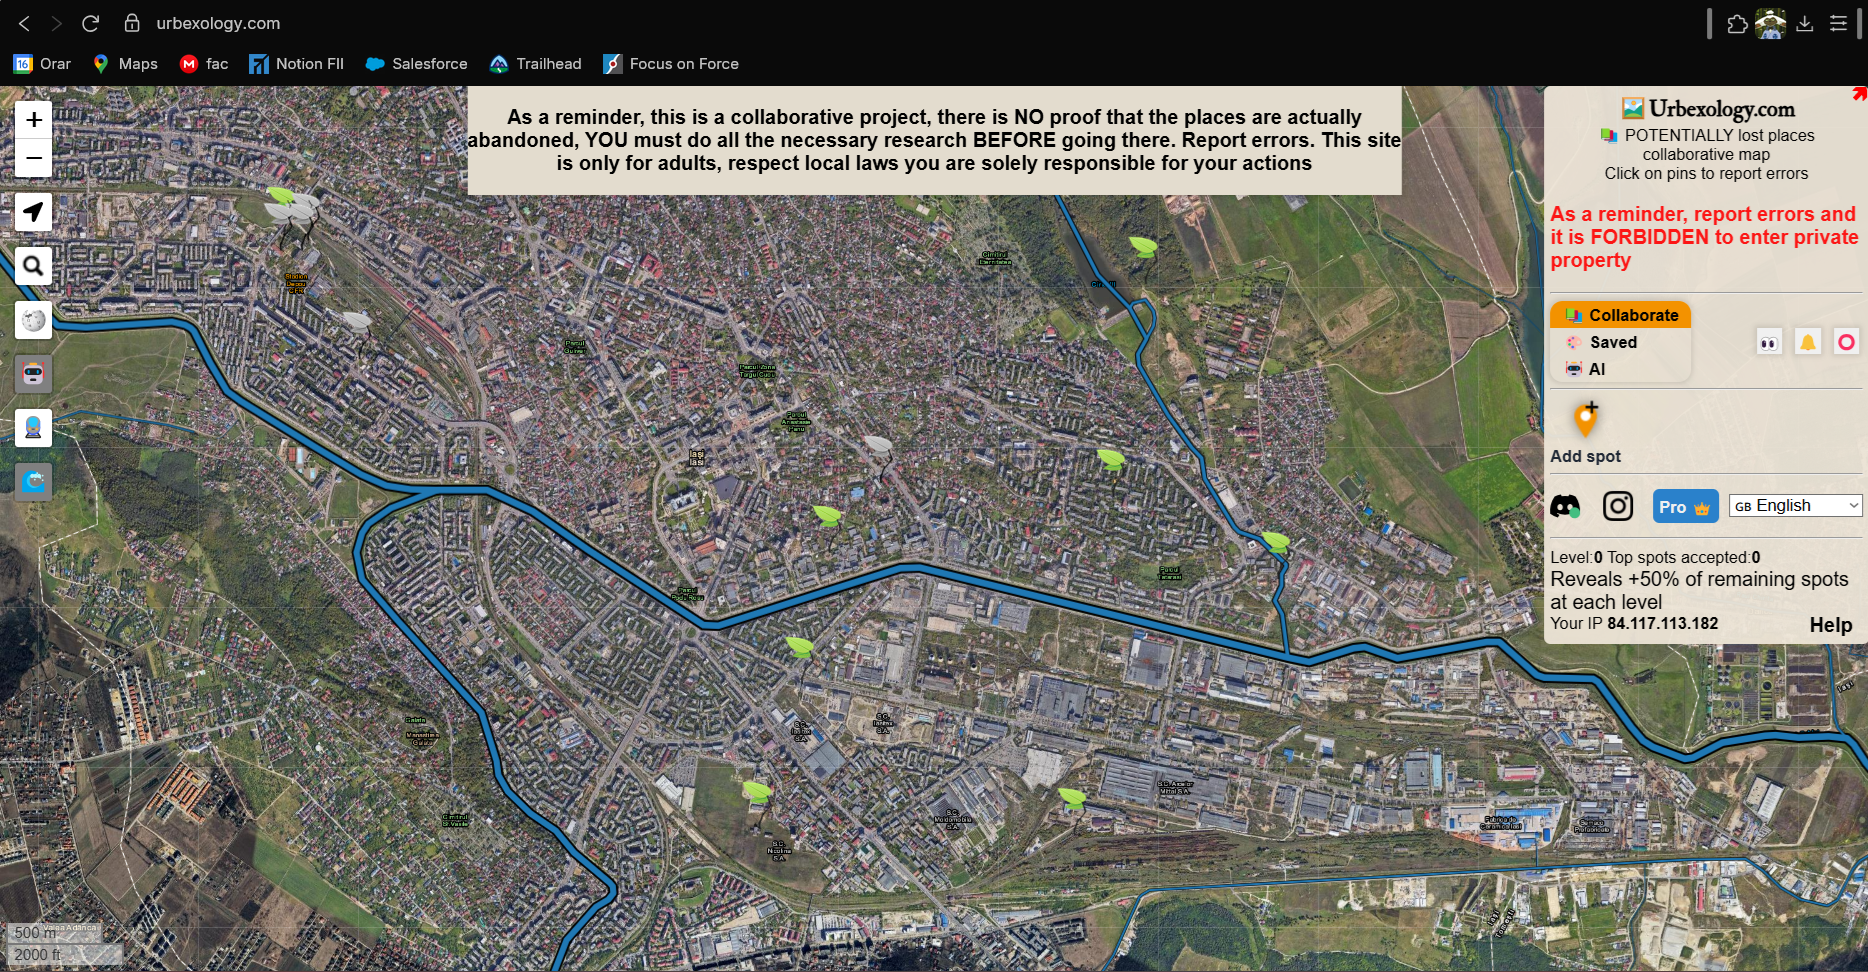
\includegraphics[width=0.8\textwidth]{images/urbexology.png}
\end{center}

In terms of romanian locations, it performs much better than the mobile app alternative, however, again, there is no automation in terms of adding locations to the map via Google. A level up system does exist, but it is more limited, in the sense that you level up by submitting locations, but not exploring them yourself, meaning people would feel less motivated to go to existing locations and add pictures or detailed descriptions.

\section{Technology Stack Analysis}
\subsection{Mapping Solutions Comparison}

The mapping technology is obviously very important since it is the core of a platform such as this one. There are many options out there for embedding a functioning map to a website, the main ones being Google Maps and Leaflet with OpenStreetMap.

Google Maps is the top player, being controlled by a tech behemoth, with the best and most varied location data in the world. But, there is always a downside. Using Google Maps' services becomes expensive after repeated usage and, on top of that, customisability is limited.

After looking at both, I chose to combine the both of them, in order to get very accurate locations from Google Maps and, at the same time, a nice looking map UI for the user.

\subsection{Backend Technologies Evaluation}
When looking at the backend technology, the choice was much easier, since I am familiar with creating a web application because of a course from the faculty of computer science. 

Node.js is something that was used on a previous project and it is extremely capable, yet not overcomplicated. On top of that, Express is perfect for creating websites as it simplifies the development process.

MongoDB was picked as opposed to any other database because of its flexbility in terms of storing data. It is much easier to work with JSON-like records instead of fields in tables. This proved very useful in the process of creating the application because necessary fields that were not added at first were added on the way.

\section{Gap Analysis}
After this much research on the topic, it is clear that existing similar platforms do not provide nearly enough content for users, neither do they present details like access information or safety head-up's. 

What Off Course wants to further add new in terms of the urbex market is the game-like system and the Google Places API automation.

For this platform to be successful in terms of data, some matter of time will need to pass since it is built mainly on user suggestions, feedback and information but I believe, with time, it will be possible with a smaller, yet dedicated fan base, since it will basically tackle most issues of the user generated content models:"User-generated content (UGC) has the potential to be diverse and authentic, but it also comes with challenges related to its accuracy, relevance, and professionalism. Since UGC is created by individuals who may have a different level of expertise or understanding than the brand, there can be variations in the quality of content produced."~\cite{ugcChallenges}


\chapter{Requirements Analysis and System Design}
\section{Functional Requirements}
\subsection{User Management}
When connecting to the website, a user is required to sign up or log in to an account, otherwise, no information will be accessible (other than the about us page, of course).

After being prompted to log in, the user information is saved to the database according to the model. 

\begin{center}
\includegraphics[width=1\textwidth]{images/user db.png}
\end{center}

As obvious from the example image, users' sensitive data is hashed for privacy and only required data is collected. As well as that, by using MongoDB, each creation request can be completed.

After creating a user record, each customer can view their profile with information about them and what they have achieved on the platform, as well as have access to all of the basic operations, like logging out, viewing locations and leaderboards and sending requests.

*It is important to mention that as the platform grows in numbers, an "admin" user feature should be implemented, in order to allow users to register or delete users that should be banned from accessing the service in the future.

\subsection{Location Management}
Locations are the most important feature of the platform, so it makes sense that a lot of information is stored about them in the database and also available to view when clicking on a spot's marker.

The two main sources of improving the website with more locations are the automatic search by Google Places API and the user submitted requests of trusted individuals, including myself and my friends.

Coordinates and other details will only be displayed for users to actually see after the request has been personally validated to make sure it is a real location and the descriptions are accurate. 

\subsection{Gamification System}
The gamification system is inspired by a lot of popular apps, games(Pokemon GO) or other types alike(Duolingo), that reward the user when completing tasks.

Experience points can be gained by visiting a location on the map, writing a review about a location you have visited and uploading relevant pictures. This helps the platform improve the quality of its content, but also make the players feel like they are actively participating and get rewarded for it.

After enough experience points are given to a player, his level increases, but the higher your level is, the more experience points you will need to level up.

This also creates a fun way to see who in the community is the most active via the leaderboard section and this can also determine people to meet other like-minded explorers and create new connections.

\subsection{Social Features}
The social features are, at the moment limited, but for a good reason. The platform will work very closely to the already existing dedicated Discord server, where a sense of community already exists. That is why I believe that adding social features to the application was not a priority.

\section{Non-Functional Requirements}
\subsection{Performance Requirements}
The website is not a service that requires a lot of processing power, neither on the client side, nor on the server side. Because the amount of locations that have to be loaded is not very high and also the amount of users will not go over the hundreds, the website is great in terms of performance.

This is convienient also for people that log onto it from their phone, since computers and laptops are faster, yet will be less used by the usual user.

\subsection{Security Requirements}
Security for the website is very strong thanks to the technologies that it makes use of.

-JWT is amazing for cookie sessions, retrieving relevant user data and redirecting people that should have no access from a specific page.
"JSON Web Token (JWT) defines a compact and self-contained way for securely transmitting information between parties as a JSON object. This information can be verified and trusted because it is digitally signed."~\cite{JWT}

-bcrypt hashes the users' passwords so their information remains private and impossible to break:
"bcrypt was designed based on the Blowfish cipher: b for Blowfish and crypt for the name of the hashing function used by the UNIX password system. [...] bcrypt forces you to follow security best practices as it requires a salt as part of the hashing process. Hashing combined with salts protects you against rainbow table attacks"~\cite{bcrypt}

-the invite system will ensure only people that have been invited can actually create an account and use the platform

\subsection{Usability Requirements}
The platform is modern so using it is very intuitive. It looks clean, with buttons that indicate what each of them does and tabs on the UI for going inbetween pages. The application is also responsive on mobile and it can also be easily used there.

\subsection{Scalability Requirements}
As mentioned before, at the performance subsection, the website will never reach extremely high numbers in terms of locations or users (estimates: 200-500 users and 300-600 locations at maximum), meaning that the current technologies that are implemented are enough to handle any operations in the future ahead.

If need be, a transfer from the raspberry pi to the cloud could be a possibility in order to reach better performance for a lot of activity.

\section{System Architecture}
\subsection{Overall Architecture}
The architecture of the website is entirely based on the MVC model which has been, for many years, considered to be the best solution for building web applications: "Originally conceptualized for desktop graphical user interfaces, MVC has evolved to become a cornerstone framework guiding the  development  of  web  and  mobile  applications.  Its  ability  to  separate  concerns—dividing  the application logic into three  interconnected  components:  the model, the view, and the  controller—facilitates  not  only  enhanced  code  reuse  but  also  parallel  development  across  teams.  This architectural  pattern  enables developers  to  manage complex  applications  efficiently, making  it  a popular choice among a wide array of industries."~\cite{mvcThesis}

Below is a simplified C4 diagram to show the main business flow of the app, especially the MVC components and REST-ful API communication:

\begin{center}
\includegraphics[width=0.8\textwidth]{images/licenta.drawio.png}
\end{center}

\subsection{Frontend Architecture}
% [To be written by student]

\subsection{Backend Architecture}
% [To be written by student]

\subsection{Database Design}
% [To be written by student]

\chapter{Technology Stack and Implementation}
\section{Technology Selection Rationale}
\subsection{Frontend Technologies}
% [To be written by student - HTML5/CSS3, JavaScript, Leaflet, Axios]

\subsection{Backend Technologies}
% [To be written by student - Node.js, Express.js, bcrypt, JWT, multer, CORS, dotenv]

\subsection{Database and External Services}
% [To be written by student - MongoDB, Google Maps API, Google Places API]

\section{System Implementation}
\subsection{Database Schema Implementation}
% [To be written by student - Complete MongoDB schemas]

\subsection{API Endpoints Design}
% [To be written by student - All REST endpoints with examples]

\subsection{Authentication Implementation}
% [To be written by student - JWT and bcrypt implementation]

\subsection{File Upload Implementation}
% [To be written by student - Multer configuration and usage]

\section{Frontend Implementation Details}
\subsection{Map Integration}
% [To be written by student - Leaflet + Google Maps implementation]

\subsection{API Communication}
% [To be written by student - Axios implementation and configuration]

\chapter{Testing and Validation}
\section{Testing Strategy}
\subsection{Unit Testing}
% [To be written by student]

\subsection{Integration Testing}
% [To be written by student]

\subsection{User Acceptance Testing}
% [To be written by student]

\section{Test Cases Implementation}
% [To be written by student]

\section{Performance Testing Results}
% [To be written by student]

\section{User Feedback and Iterations}
% [To be written by student]

\chapter{Deployment and Hosting}
\section{Hosting Solution}
\subsection{Raspberry Pi Deployment}
% [To be written by student]

\subsection{Domain and DNS Configuration}
% [To be written by student]

\section{Production Environment Setup}
% [To be written by student]

\section{Monitoring and Maintenance}
% [To be written by student]

% Conclusions
\chapter*{Conclusions}
\addcontentsline{toc}{chapter}{Conclusions}

\section*{Main Contributions}
% [To be written by student]

\section*{Objectives Achievement Analysis}
% [To be written by student]

\section*{Lessons Learned}
% [To be written by student]

\section*{Future Work and Improvements}
% [To be written by student]

\bibliographystyle{IEEEtran}
\bibliography{references}

% Appendices
\appendix
\chapter{Code Samples}
% [To be written by student]

\chapter{Database Schema}
% [To be written by student]

\chapter{API Documentation}
% [To be written by student]

\chapter{User Interface Screenshots}
% [To be written by student]

\chapter{Test Results}
% [To be written by student]

\end{document}